\documentclass[11pt, oneside]{article}
\usepackage{geometry}
\usepackage{graphicx}
\usepackage{amssymb}
\usepackage{amsmath}
\usepackage[
  backend=bibtex,
  style=numeric,
  sorting=none,
  citestyle=numeric-comp
]{biblatex}
\addbibresource{references.bib}

\geometry{letterpaper}

\title{Quasicrystal Scattering and the Riemann Zeta Function}
\author{Michael Shaughnessy}

\begin{document}
\maketitle

\begin{abstract}
We investigate one-dimensional scattering from a quasicrystal-like atomic arrangement, $\chi(x)$, derived from prime number positions with a shift operation to achieve approximately constant density. Numerical scattering calculations reveal peaks in the scattering amplitude aligning with the imaginary parts of the non-trivial zeros of the Riemann Zeta Function (RZF). An analytic computation, including a simple crystal example and contour integration via the residue theorem, confirms that these peaks arise from poles at RZF zeros. This work bridges number theory and wave scattering, offering a physical interpretation of RZF zeros as scattering resonances.
\end{abstract}

\section{Introduction}

The Riemann Zeta Function (RZF) connects the distribution of prime numbers to its non-trivial zeros, a relationship explored since Riemann’s 1859 work showing primes are ordered but non-periodic \cite{Riemann1859}. Von Mangoldt’s 1895 explicit formula linked prime powers to RZF zeros \cite{VonMangoldt1895}, and the Guinand-Weil formula expresses the Fourier transform of RZF zeros as a sum over prime powers \cite{Weil}:

\begin{equation}
\sum_{\rho} h(\rho) = h(0) + h(1) - \sum_{p} \sum_{m=1}^{\infty} \frac{h(\log p^m)}{p^{m/2}} \log p - \int_{-\infty}^{\infty} \frac{h(t) \Phi(t)}{2} dt
\end{equation}

Freeman Dyson proposed that quasicrystals—ordered, non-periodic structures observed by Shechtman in 1984 \cite{Shechtman1984}—might elucidate the RZF zeros’ structure \cite{Baez2013}. Inspired by this, we construct a one-dimensional potential, $\chi(x)$, from prime number positions normalized to constant density. We demonstrate that its scattering amplitude exhibits peaks at the imaginary parts of RZF zeros, linking number theory to physical scattering processes.

\subsection{Fourier Transform and Scattering}

Scattering involves computing the Fourier transform of a potential $V(x)$ to obtain the scattering amplitude $\hat{V}(k)$:

\begin{equation}
\hat{V}(k) = \int_{-\infty}^{\infty} V(x) e^{-i k x} dx
\end{equation}

For a potential $V(x) = \sum_{x_n \in X} \delta(x - x_n)$, where $\delta(x)$ is the Dirac delta function, the Fourier transform may be a tempered distribution:

\begin{equation}
\hat{V}(k) = \hat{h}(k) + \sum_{k_m \in X^{*}} \hat{V}_{m} \delta(k - k_m)
\end{equation}

If $\hat{h}(k) = 0$, $V(x)$ is a quasicrystal, and the double Fourier transform recovers $V(x)$. We define:

\begin{equation}
V(x) = \sum_{p \text{ prime}} \delta(x - p)
\end{equation}

and apply a shift operation to create $\chi(x)$, mapping prime positions $p_n$ to $p_n \cdot \frac{1}{\pi(p_n)} \approx \log p_n$, where $\pi(x)$ is the prime counting function. This normalization ensures approximately constant atomic density (which is the physical requirement for a well-defined scattering spectrum), facilitating the connection to RZF zeros via the logarithmic distribution of primes.

\section{Numerical Supercell Method and Results}

\subsection{Method}

The planewave basis supercell method is a numerical technique for approximating a finite system with an infinite periodic crystalline structure. It is well-suited for calculations of physical properties of materials having 1.) finite spacing between atoms and 2.) long range order of atomic positions, meaning atomic locations are not completely random, ie being a homogenous material with well-defined bulk properties.
  
We compute and present scattering amplitudes for finite-length supercell approximations of $\chi(x)$, parameterized by the number of atoms in the supercell, $L_{\chi}$. The starting potential is:

\begin{equation}
\chi(x) = \sum_{p \text{ prime}} \delta(x - \log p)
\end{equation}

Prime positions are shifted using $p_n \cdot \frac{1}{\pi(p_n)} \approx \log p_n$, normalizing density (see Figure \ref{fig:normalized_positions}).

\begin{figure}[htbp]
\centering
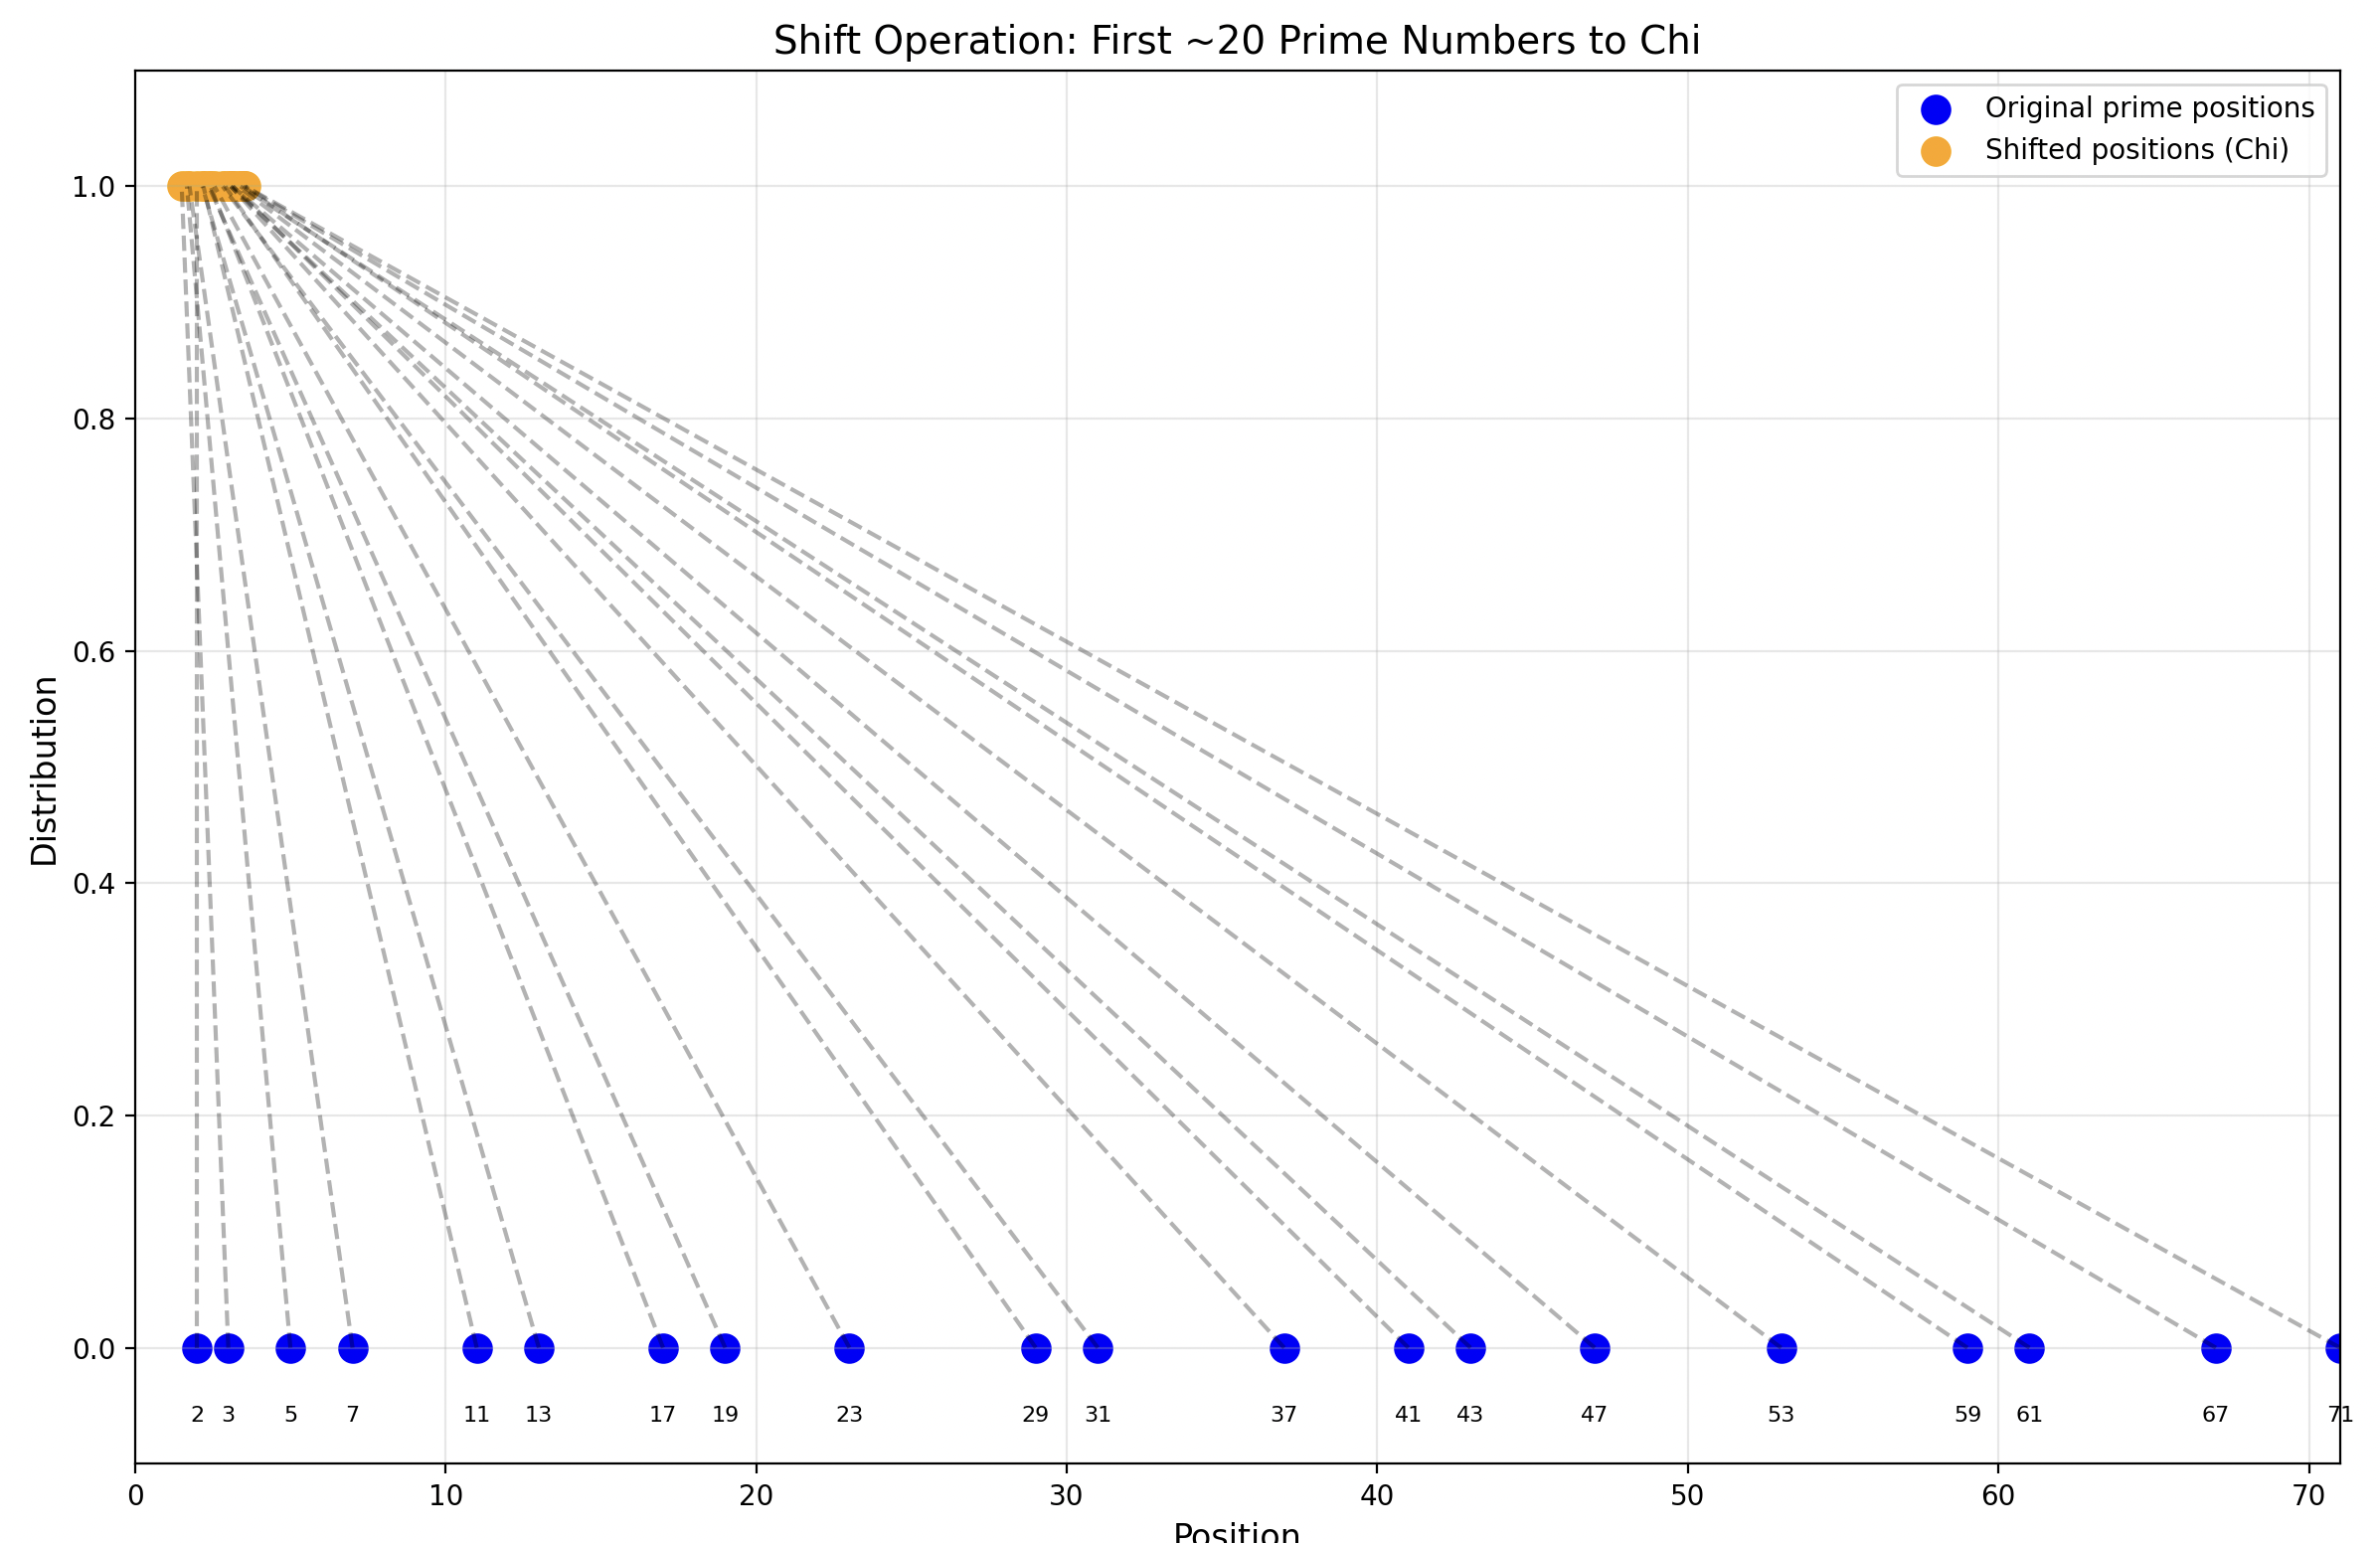
\includegraphics[width=0.8\linewidth]{normalizing.png}
\caption{Un-normalized (blue) and normalized (yellow) atomic positions in $\chi(x)$, illustrating the shift to constant density.}
\label{fig:normalized_positions}
\end{figure}

Calculations employ a one-dimensional plane-wave basis for supercell potentials $[\chi_L(x)]$. Code is available at:

\url{https://github.com/mickeyshaughnessy/quasicrystal/blob/main/scattering.py}

\subsection{Results}

The scattering amplitude shows peaks at $k$ values corresponding to the imaginary parts of RZF non-trivial zeros, with amplitude decaying as momentum increases (see Figure \ref{fig:scattering_amplitude}).

\begin{figure}[htbp]
\centering
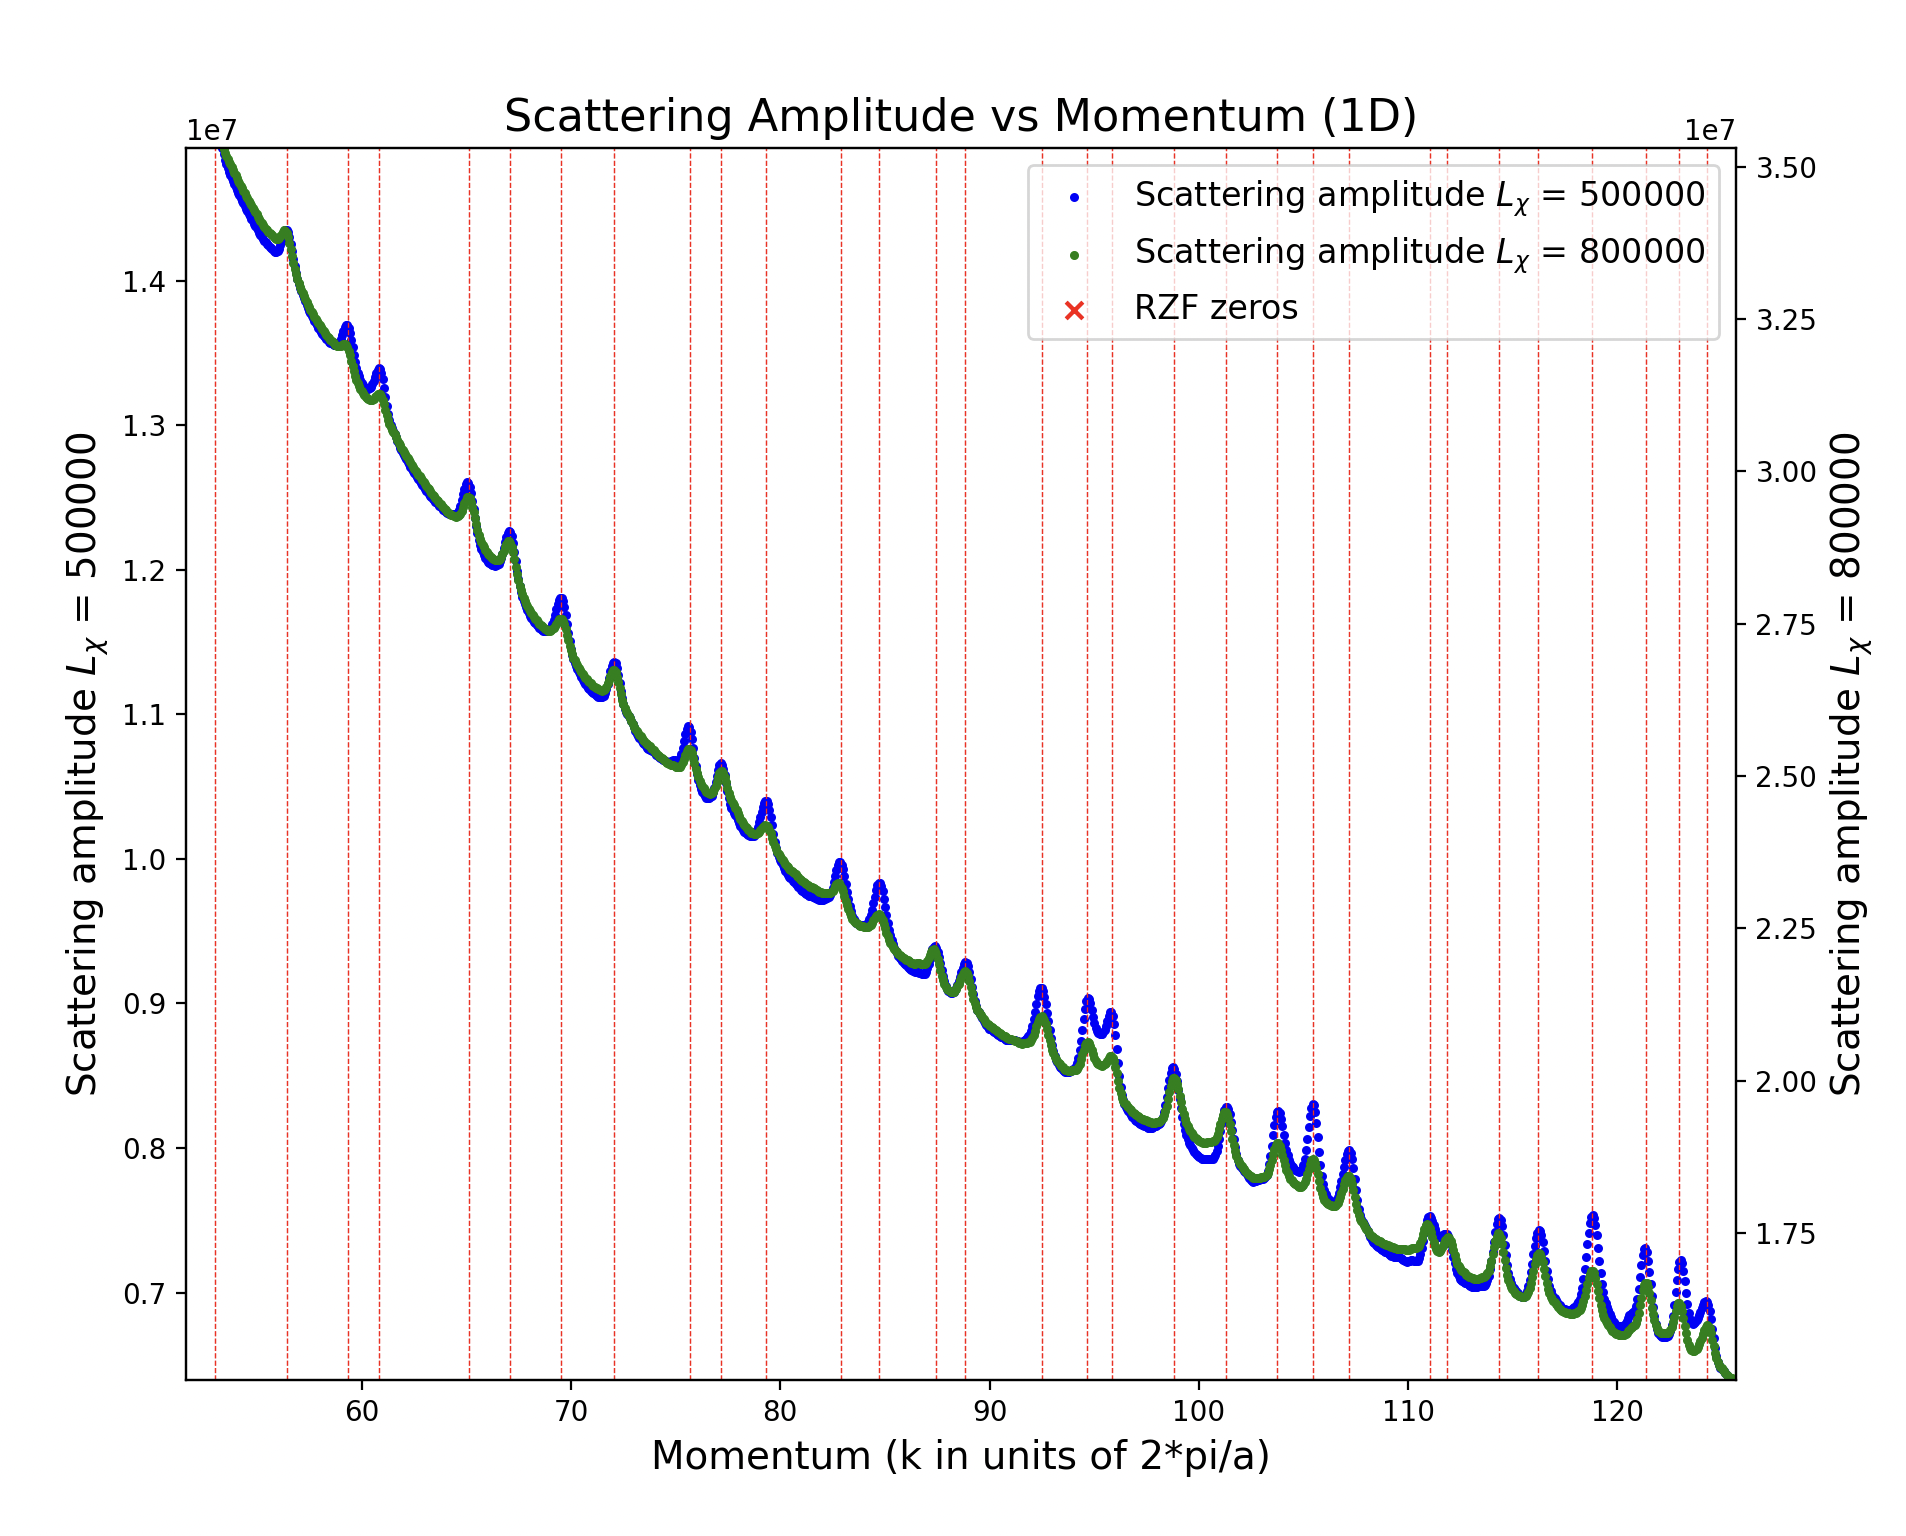
\includegraphics[width=0.8\linewidth]{zoomed_scattering.png}
\caption{Scattering amplitude for finite $L_{\chi}$, with vertical red lines marking the locations of the imaginary parts of RZF non-trivial zeros.}
\label{fig:scattering_amplitude}
\end{figure}

Key findings include:
1. Peaks align closely with RZF zeros, indicating a direct correspondence.
2. The peak-and-trough pattern persists across $L_{\chi}$ values, confirming robustness.
3. The amplitude’s structure reflects the influence of RZF zeros on scattering dynamics.

\section{Analytic Computation with Residue Theorem}

We analytically compute the Fourier transform of $\chi(x)$ using contour integration and the residue theorem. To illustrate the method, we first analyze a simple crystal with delta functions at positive integers, then apply the technique to $\chi(x)$.

\subsection{Simple Crystal Example}

Consider a one-dimensional crystal with density:

\begin{equation}
\rho(x) = \sum_{n=1}^{\infty} \delta(x - n)
\end{equation}

Its Fourier transform is:

\begin{equation}
\hat{\rho}(k) = \int_{-\infty}^{\infty} \rho(x) e^{-ikx} dx = \sum_{n=1}^{\infty} e^{-ikn}
\end{equation}

This geometric series, with ratio $e^{-ik}$ ($|e^{-ik}| = 1$), diverges for real $k$. We introduce a convergence factor $e^{-\epsilon n}$:

\begin{equation}
\hat{\rho}(k) = \lim_{\epsilon \to 0^+} \sum_{n=1}^{\infty} e^{-ikn} e^{-\epsilon n} = \lim_{\epsilon \to 0^+} \frac{e^{-ik-\epsilon}}{1 - e^{-ik-\epsilon}} = \frac{1}{e^{ik} - 1}
\end{equation}

Using contour integration, consider:

\begin{equation}
f(z) = \frac{e^{-ikz}}{1 - e^{-2\pi i z}}
\end{equation}

This has simple poles at $z = n$ (integers $n$), with residues:

\begin{equation}
\text{Res}[f, n] = \lim_{z \to n} (z - n) \frac{e^{-ikz}}{1 - e^{-2\pi i z}} = \frac{e^{-ikn}}{2\pi i}
\end{equation}

We integrate over a contour $C$ from $R$ to $R+i$, $R+i$ to $\epsilon+i$, $\epsilon+i$ to $\epsilon$, and $\epsilon$ to $R$, taking $R \to \infty$ and $\epsilon \to 0^+$. The residue theorem gives:

\begin{equation}
\oint_C f(z) dz = 2\pi i \sum_{n=1}^{\lfloor R \rfloor} \frac{e^{-ikn}}{2\pi i} = \sum_{n=1}^{\lfloor R \rfloor} e^{-ikn}
\end{equation}

As $R \to \infty$, this yields $\sum_{n=1}^{\infty} e^{-ikn}$. Evaluating the contour, horizontal segments cancel, and vertical segments confirm $\hat{\rho}(k) = \frac{1}{e^{ik} - 1}$. At $k = 2\pi m$ ($m \neq 0$), singularities produce Bragg peaks, characteristic of crystalline diffraction.

This analysis demonstrates the fundamental principle of crystallography: the Fourier transform of a periodic structure consists of discrete peaks in reciprocal space. 

\subsection{Analysis of $\chi(x)$}

For the quasicrystal potential:

\begin{equation}
\chi(x) = \sum_{p \in P} \delta(x - \log p)
\end{equation}

The Fourier transform is:

\begin{equation}
\hat{\chi}(k) = \sum_{p \in P} p^{-ik}
\end{equation}

This resembles the logarithmic derivative of the RZF, $-\frac{\zeta'(s)}{\zeta(s)} = \sum_{n=1}^\infty \Lambda(n) n^{-s}$, where $\Lambda(n)$ is the von Mangoldt function. To ensure convergence, we introduce $p^{-\epsilon}$:

\begin{equation}
S_\epsilon(k) = \sum_{p \in P} p^{-\epsilon - ik}
\end{equation}

We express this as a contour integral:

\begin{equation}
S_\epsilon(k) = \frac{1}{2\pi i} \int_{c - i \infty}^{c + i \infty} -\frac{\zeta'(s)}{\zeta(s)} \cdot \frac{1}{s - (\epsilon + ik)} ds
\end{equation}

where $c > 1$. Poles occur at RZF zeros $\rho$ and at $s = \epsilon + ik$. The residue theorem yields:

\begin{equation}
S_\epsilon(k) = \sum_{\rho} \frac{1}{\rho - (\epsilon + ik)} + \frac{\zeta'(\epsilon + ik)}{\zeta(\epsilon + ik)}
\end{equation}

As $\epsilon \to 0$:

\begin{equation}
S(k) = \sum_{\rho} \frac{1}{\rho - ik} + \frac{\zeta'(ik)}{\zeta(ik)}
\end{equation}

Poles at $\rho$ produce peaks in $\hat{\chi}(k)$ at $k = \text{Im}(\rho)$, matching numerical results.

\subsection{Summary}

The simple crystal example demonstrates how contour integration yields a Fourier transform with discrete peaks. For $\chi(x)$, the residue theorem shows that RZF zeros contribute poles to $\hat{\chi}(k)$, causing resonances at $k = \text{Im}(\rho)$. This explains the observed peaks, linking the analytic structure to numerical results.

\section{Conclusion}

This study establishes a novel connection between the RZF and wave scattering from a quasicrystal-like potential $\chi(x)$. Numerical scattering amplitudes exhibit robust peaks at the imaginary parts of RZF non-trivial zeros. Analytic computations, including a simple crystal example, confirm that these peaks arise from poles at RZF zeros in the Fourier transform of $\chi(x)$. By interpreting RZF zeros as scattering resonances, this work offers a physical perspective on a fundamental mathematical object. Future research could explore higher-dimensional quasicrystals, alternative density normalization methods, or experimental realizations of such scattering systems to further probe this connection.

\section{Acknowledgements}
I gratefully acknowledge discussions with C.Y. Fong, John Baez, Jamison Galloway, Robert Hayre, Chun Yen Lin, Charles Martin, Aftab Ahmed, Catalin Spataru, Naveen Ashok, various LLMs including Grok, Claude, and ChatGPT; and anonymous contributors on X. C. Y. Fong also provided the original planewave supercell scattering code.

\printbibliography

\end{document}